\documentclass[11pt]{article}
\usepackage{geometry}                % See geometry.pdf to learn the layout options. There are lots.
\geometry{letterpaper}                   % ... or a4paper or a5paper or ... 
%\geometry{landscape}                % Activate for for rotated page geometry
%\usepackage[parfill]{parskip}    % Activate to begin paragraphs with an empty line rather than an indent
\usepackage{graphicx}
\usepackage{amssymb,amsmath}
\usepackage{epstopdf}
\usepackage{pgf}
\usepackage{pgfpages}
\usepackage{tikz}
\usetikzlibrary{arrows,backgrounds}
\usepgflibrary{shapes}
\DeclareGraphicsRule{.tif}{png}{.png}{`convert #1 `dirname #1`/`basename #1 .tif`.png}
\pagestyle{empty}


\begin{document}
  \begin{center}
   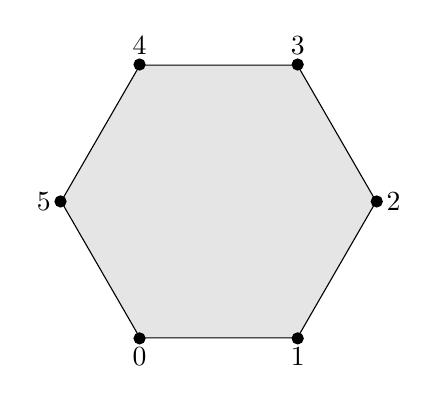
\begin{tikzpicture}
      \node[name=p6, regular polygon,regular polygon sides=6, minimum size=4cm, draw, fill=black!10]{};
      \filldraw(p6.corner 1) circle (2pt);
      \filldraw(p6.corner 2) circle (2pt);
      \filldraw(p6.corner 3) circle (2pt);
      \filldraw(p6.corner 4) circle (2pt);
      \filldraw(p6.corner 5) circle (2pt);
      \filldraw(p6.corner 6) circle (2pt);
      \node[left] at (p6.corner 3){5};
      \node[below] at (p6.corner 4){0};
      \node[below] at (p6.corner 5){1};
      \node[above] at (p6.corner 1){3};
      \node[above] at (p6.corner 2){4};
      \node[right] at (p6.corner 6){2};
    \end{tikzpicture}
    \hspace{2cm}
    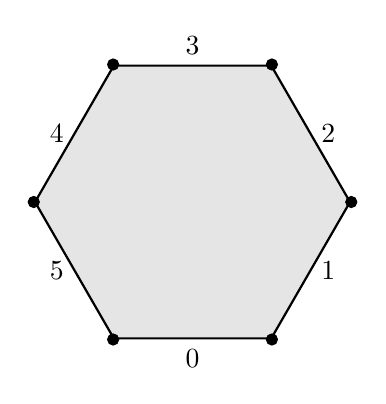
\begin{tikzpicture}
      \node[name=p6, regular polygon,regular polygon sides=6, minimum size=4cm, draw, thick, fill=black!10]{};
      \filldraw(p6.corner 1) circle (2pt);
      \filldraw(p6.corner 2) circle (2pt);
      \filldraw(p6.corner 3) circle (2pt);
      \filldraw(p6.corner 4) circle (2pt);
      \filldraw(p6.corner 5) circle (2pt);
      \filldraw(p6.corner 6) circle (2pt);
      \node[left] at (p6.side 3){5};
      \node[below] at (p6.side 4){0};
      \node[right] at (p6.side 5){1};
      \node[above] at (p6.side 1){3};
      \node[left] at (p6.side 2){4};
      \node[right] at (p6.side 6){2};
    \end{tikzpicture}
  \end{center}
 \begin{center} 
     \hspace{1cm} (a) \hspace{5cm} (b)  \\
 \end{center}

\end{document}  
